% !TEX TS-program = knitr
\documentclass{article}\usepackage{graphicx, color}
%% maxwidth is the original width if it is less than linewidth
%% otherwise use linewidth (to make sure the graphics do not exceed the margin)
\makeatletter
\def\maxwidth{ %
  \ifdim\Gin@nat@width>\linewidth
    \linewidth
  \else
    \Gin@nat@width
  \fi
}
\makeatother

\IfFileExists{upquote.sty}{\usepackage{upquote}}{}
\definecolor{fgcolor}{rgb}{0.2, 0.2, 0.2}
\newcommand{\hlnumber}[1]{\textcolor[rgb]{0,0,0}{#1}}%
\newcommand{\hlfunctioncall}[1]{\textcolor[rgb]{0.501960784313725,0,0.329411764705882}{\textbf{#1}}}%
\newcommand{\hlstring}[1]{\textcolor[rgb]{0.6,0.6,1}{#1}}%
\newcommand{\hlkeyword}[1]{\textcolor[rgb]{0,0,0}{\textbf{#1}}}%
\newcommand{\hlargument}[1]{\textcolor[rgb]{0.690196078431373,0.250980392156863,0.0196078431372549}{#1}}%
\newcommand{\hlcomment}[1]{\textcolor[rgb]{0.180392156862745,0.6,0.341176470588235}{#1}}%
\newcommand{\hlroxygencomment}[1]{\textcolor[rgb]{0.43921568627451,0.47843137254902,0.701960784313725}{#1}}%
\newcommand{\hlformalargs}[1]{\textcolor[rgb]{0.690196078431373,0.250980392156863,0.0196078431372549}{#1}}%
\newcommand{\hleqformalargs}[1]{\textcolor[rgb]{0.690196078431373,0.250980392156863,0.0196078431372549}{#1}}%
\newcommand{\hlassignement}[1]{\textcolor[rgb]{0,0,0}{\textbf{#1}}}%
\newcommand{\hlpackage}[1]{\textcolor[rgb]{0.588235294117647,0.709803921568627,0.145098039215686}{#1}}%
\newcommand{\hlslot}[1]{\textit{#1}}%
\newcommand{\hlsymbol}[1]{\textcolor[rgb]{0,0,0}{#1}}%
\newcommand{\hlprompt}[1]{\textcolor[rgb]{0.2,0.2,0.2}{#1}}%

\usepackage{framed}
\makeatletter
\newenvironment{kframe}{%
 \def\at@end@of@kframe{}%
 \ifinner\ifhmode%
  \def\at@end@of@kframe{\end{minipage}}%
  \begin{minipage}{\columnwidth}%
 \fi\fi%
 \def\FrameCommand##1{\hskip\@totalleftmargin \hskip-\fboxsep
 \colorbox{shadecolor}{##1}\hskip-\fboxsep
     % There is no \\@totalrightmargin, so:
     \hskip-\linewidth \hskip-\@totalleftmargin \hskip\columnwidth}%
 \MakeFramed {\advance\hsize-\width
   \@totalleftmargin\z@ \linewidth\hsize
   \@setminipage}}%
 {\par\unskip\endMakeFramed%
 \at@end@of@kframe}
\makeatother

\definecolor{shadecolor}{rgb}{.97, .97, .97}
\definecolor{messagecolor}{rgb}{0, 0, 0}
\definecolor{warningcolor}{rgb}{1, 0, 1}
\definecolor{errorcolor}{rgb}{1, 0, 0}
\newenvironment{knitrout}{}{} % an empty environment to be redefined in TeX

\usepackage{alltt}

\usepackage{amsfonts}
\usepackage{amsmath}
\usepackage{amssymb}
\usepackage{amsthm}
\usepackage{caption}
\usepackage{color}
\usepackage{enumerate}
\usepackage{fancyhdr}
\usepackage{hyperref}
\usepackage{graphicx}
\usepackage{latexsym}
\usepackage{listings}
\usepackage{mathrsfs}
\usepackage{natbib}
\usepackage[nottoc]{tocbibind}
\usepackage{url}

\providecommand{\all}{\ \forall \ }
\providecommand{\bs}{\backslash}
\providecommand{\e}{\varepsilon}
\providecommand{\E}{\ \exists \ }
\providecommand{\lm}[2]{\lim_{#1 \rightarrow #2}}
\providecommand{\m}[1]{\mathbb{#1}}
\providecommand{\nv}{{}^{-1}}
\providecommand{\ov}[1]{\overline{#1}}
\providecommand{\p}{\newpage}
\providecommand{\q}{$\quad$ \newline}
\providecommand{\rt}{\rightarrow}
\providecommand{\Rt}{\Rightarrow}
\providecommand{\vc}[1]{\boldsymbol{#1}}
\providecommand{\wh}[1]{\widehat{#1}}

%\renewcommand\bibname{References}
%\renewcommand{\thesection}{Problem \arabic{section}}
%\renewcommand{\thesubsection}{Part \alph{subsection}}
\numberwithin{equation}{section}

\fancyhead{}
\fancyfoot{}
\fancyhead[R]{\thepage}
\fancyhead[C]{Landau}

\hypersetup{
    colorlinks,
    citecolor=black,
    filecolor=black,
    linkcolor=black,
    urlcolor=blue
}

\definecolor{dkgreen}{rgb}{0,0.6,0}
\definecolor{gray}{rgb}{0.5,0.5,0.5}
\definecolor{mauve}{rgb}{0.58,0,0.82}

\lstset{ 
  language=C,                % the language of the code
  basicstyle=\Large,           % the size of the fonts that are used for the code
  numberstyle= \tiny \color{white},  % the style that is used for the line-numbers
  stepnumber=2,                   % the step between two line-numbers. 
  numbersep=5pt,                  % how far the line-numbers are from the code
  backgroundcolor=\color{white},      % choose the background color. You must add \usepackage{color}
  showspaces=false,               % show spaces adding particular underscores
  showstringspaces=false,         % underline spaces within strings
  showtabs=false,                 % show tabs within strings adding particular underscores
  frame=lrb,                   % adds a frame around the code
  rulecolor=\color{black},        % if not set, the frame-color may be changed on line-breaks within not-black text 
  tabsize=2,                      % sets default tabsize to 2 spaces
  captionpos=t,                   % sets the caption-position 
  breaklines=true,                % sets automatic line breaking
  breakatwhitespace=false,        % sets if automatic breaks should only happen at whitespace
  title=\lstname,                   % show the filename of files included with \lstinputlisting;
  keywordstyle=\color{blue},          % keyword style
  commentstyle=\color{gray},       % comment style
  stringstyle=\color{dkgreen},         % string literal style
  escapeinside={\%*}{*)},            % if you want to add LaTeX within your code
  morekeywords={*, ...},               % if you want to add more keywords to the set
  xleftmargin=0.053in, % left horizontal offset of caption box
  xrightmargin=-.03in % right horizontal offset of caption box
}

\DeclareCaptionFont{white}{\color{white}}
\DeclareCaptionFormat{listing}{\parbox{\textwidth}{\colorbox{gray}{\parbox{\textwidth}{#1#2#3}}\vskip-0.05in}}
\captionsetup[lstlisting]{format = listing, labelfont = white, textfont = white}
% For caption-free listings, comment out the 3 lines above and uncomment the 2 lines below.
% \captionsetup{labelformat = empty, labelsep = none}
% \lstset{frame = single}






\begin{document}



\begin{flushleft}


\begin{center} \LARGE
STAT 305 D Homework 2 
\end{center}
\begin{center} \Large
Due January 31, 2012 at 12:40 PM in class
\end{center}


\begin{enumerate}[1. ]
\item Vardeman and Jobe Chapter 1 Exercise 2 (page 23): If factor A has levels 1, 2, and 3, factor B has levels 1 and 2, and factor C has levels 1 and 2, list the combinations of A, B, and C that make up a full factorial arrangement.
\item Vardeman and Jobe Chapter 1 Exercise 10 (page 24): Give an example of a 2 $\times$ 3 full factorial data structure that might arise in a student study of the breaking strengths of wooden dowels. (Name the two factors involved, their levels, and write out all six different combinations. You must create the factors yourself. They are not given to you in this problem.) Then make up a data collection form for the study. Plan to record both the breaking strength and whether the break was clean or splintered for each dowel, supposing that three dowels of each type are to be tested.

\item  Vardeman and Jobe Chapter 2 Exercise 3 (page 64): 

An experiment is to be performed to compare the effects of two different methods for loading gears in a carburizing furnace on the amount of distortion produced in a heat treating process. Thrust face runout will be measured for gears laid and for gears hung while treating.

\begin{enumerate}[a. ]
\item 20 gears are to be used in the study. Randomly divide up the gears into a group (of 10) to be laid and a group (of 10) to be hung, using Table B.1 (available at \href{http://will-landau.com/stat305/tables/random-digits.pdf}{http://will-landau.com/stat305/tables/random-digits.pdf}). Describe carefully how you do this. If you use the table, begin in the upper left corner.
\item What are some purposes of the randomization used in part (a)?
\end{enumerate}


\item Now, suppose you want to distinguish between the big gears (10 of them) and the small gears (10 of them). You want to design an improved study to test the effect of gear arrangement on gear distortion. This new study takes the different gear sizes into account. (After all, small gears may distort less than big gears, or vice versa.) You plan to lay 5 small gears, hang 5 small gears, lay 5 big gears, and hang 5 big gears.

\begin{enumerate}[a. ]
\item Name the design of the study. Also, construct a table with all sample units as rows and variables as columns to show all the combinations of levels of the variables.
\item Carry out the appropriate randomization to assign the 20 gears to the appropriate treatment groups for the experiment.
\end{enumerate}




\item Vardeman and Jobe Chapter 3 Section 1 problem 1 (page 77):

\setkeys{Gin}{width=.75\textwidth} 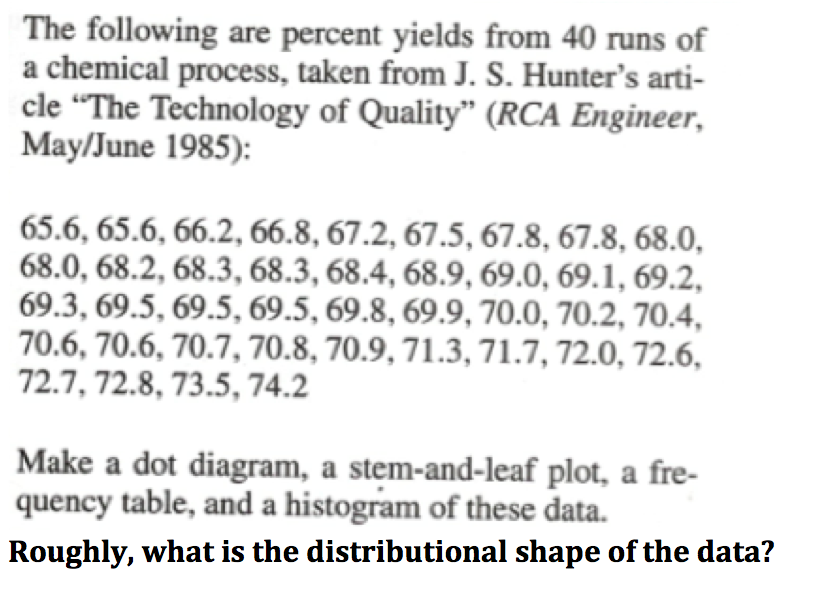
\includegraphics{../../fig/ch3s1p1.png}



\item Vardeman and Jobe Chapter 3 Section 2, part (a) of problem 1 (page 92):

\setkeys{Gin}{width=.75\textwidth} 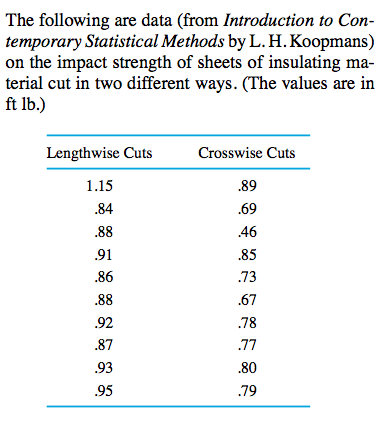
\includegraphics{../../fig/ch3s2p1.png}
Find the medians, quartiles, and the .37 quantiles of the two datasets.



\item Identify the following distributional shapes:

\setkeys{Gin}{width=.75\textwidth} 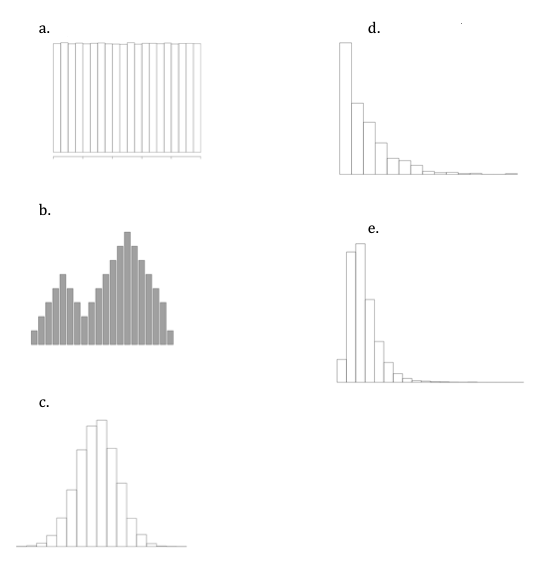
\includegraphics{../../fig/hw2shapes.png}













\item Weekly feedback. You get full credit as long as you write something.
\begin{enumerate}[1. ]
\item Is there any aspect of the subject matter that you currently struggle with? If so, what specifically do you find difficult or confusing? The more detailed you are, the better I can help you.
\item Do you have any questions or concerns about the material, class logistics, or anything else? If so, fire away.
\end{enumerate}

\end{enumerate}




\end{flushleft}
%\newpage 
%\nocite{*}
%\bibliographystyle{plainnat} 
%\bibliography{}
\end{document}
